	% abstract
\begin{abstract}¸
	The artifacts described in this document refer to the study ``\textit{Analyzing the Impact of Workloads on Modeling the Performance of Configurable Software Systems}'' which explores how configuration options can influence software performance in dependence of the workload.
	
	This document describes all artifacts accompanied with our paper.	
	Specifically, we explain the experimental setup (software configurations and workload references), measurement data (performance and code coverage), and an interactive dashboard to enable reproduction of analyses and visualizations. We make all material available via an archived software repository on \textit{zenodo.org}.
\end{abstract}

\section{Research Overview}
Software systems can be customized through configuration options to enable desired functionality or improve non-functional aspects, such as performance or energy consumption. To estimate the performance of such systems, prediction models map a given configuration to an estimated performance value~\cite{pereira_2021_learning,kaltenecker_interplay_2020}. These models are based on a training set of configuration-specific performance measurements, which usually rely on only a single workload. However, previous work shows that the choice of workload, besides configuration, can significantly influence the performance of software systems in various ways~\cite{alves_sampling_2020,lesoil_2021}.  

We conduct a systematic study that explores the quality and driving factors of the interaction between configuration options and workloads and their impact on software performance~\cite{muhlbauer_workload_2023}. In total, we analyze 25\,258 configurations and multiple workloads across nine real-world configurable software systems (\textsc{Java} and \textsc{C}/\textsc{C++}). We augment performance observations with code coverage information to explore driving causes for interactions between the workload and configuration options regarding their effect on software performance. 

The study demonstrates that workloads and configuration options may interact for performance, often in non-monotonous and non-linear ways. This result has significant implications to the generalizability of prediction models to arbitrary workloads. In addition, the observed configuration-specific sensitivity to the workload does not necessarily affect all configuration options equally, but is rather specific to individual configuration options. We identify workload-specific code coverage (i.e., code missed or covered only under specific workloads) as a partial cause for workload sensitivity.

\section{Artifacts}
To complement the representative selection of results~\cite{muhlbauer_workload_2023} and, to enable \textit{repoducibility} of our findings, we provide the experimental setup, measurement data (performance and code coverage), and our analysis implementations integrated into an interactive dashboard.

We make all material available under the open-source CC~{BY-SA~4.0 license\footnote{The full license text, explanations, and requirements of this open-source license can be found at \url{https://creativecommons.org/licenses/by-sa/4.0/}.} at \textit{zenodo.org}:
\begin{quotation}
	\url{https://doi.org/10.5281/zenodo.7504284}
\end{quotation}


\subsection{Experimental Setup}
The experimental setup comprises artifacts that are required to reproduce the experiments and obtain measurement data. 

\subsubsection{Software Configurations} For each subject system, we provide  a CSV file describing the configurations tested. Each configuration can be identified by a unique integer and specifies whether a configuration option was selected or not. 

We derived configurations from a feature model, which describes the validity constraints for each software system (i.e., which configuration options can be selected in which manner). In our study, all configuration options were binary options. In cases, where a software system also exhibited numeric options, we varied its value across, at least, two levels. We provide the feature models as DIMACS files (to use with any SAT solver) as well as XML files to be used with our sampling infrastructure \textsc{SLPConqueror}\footnote{\textsc{SPLConqueror}: \url{https://github.com/se-sic/SPLConqueror/}}. Aa summary of the sampling strategies can be found in the original paper~\cite{muhlbauer_workload_2023}.

Due to storage quota limitations (especially for raw video files) and copyright concerns (not all workloads are licensed for redistribution), we provide only a list of workloads references. 

\subsubsection{Compilation Scripts} For each \textsc{C/C++} subject system, we provide scripts to build two variants of the executable binaries with \textsc{Clang/LLVM}\footnote{Code Coverage Analysis with \textsc{Clang} and \textsc{LLVM}: \url{https://clang.llvm.org/docs/SourceBasedCodeCoverage.html}}. We build (1) binaries without any compiler optimization enabled to rule out any distortion, and (2) without compiler optimizations, but instrumentation code included to track the coverage of each line of code. 

For each \textsc{Java} subject systems, we followed their respective build instructions to obtain an executable JAR file. Unlike above, we did not weave instrumentation code into the Java code, but instead instrumented the JVM via \textsc{Jacoco}\footnote{\textsc{Jacoco}: \url{https://www.jacoco.org/jacoco/trunk/doc/}}.

\subsubsection{Measurement Scripts} In our experiment, we used the workload manager \textsc{Slurm}\footnote{\textsc{Slurm}: \url{https://slurm.schedmd.com/documentation.html}} to orchestrate and deploy experiment runs to different compute clusters. Nonetheless, the measurement scripts can be executed in isolation to obtain measurements. A hardware setup differing from the one used in our study~\cite{muhlbauer_workload_2023} will likely yield different results since the hardware specifications are likely to influence performance. 

To repeat the experiments and reproduce the performance and coverage measurements, we provide a set of scripts that we orchestrated using \textsc{Slurm}. In particular, these scripts translate the configurations provided to runtime arguments passed to the respective binaries. We used the performance analysis tool \textsc{GNU time} to record execution times and \textsc{OLTPBench}~\cite{difallah_oltp_2013} to record throughput (for the database system \htwo).


\subsection{Measurement Data}
\subsubsection{Performance Measurements} 
We provide the performance measurement data as CSV files for each subject system. Except for the database system \htwo, we report the median execution time. For \htwo, we report the throughput (transactions per second) from executing the respective combination of workload an configurations. Each data point can be identified by the unique configuration identifier and the workload name.

\subsubsection{Coverage Data}
We provide the coverage measurements in two forms. First, we provide the raw coverage reports for each combination of configuration and workload as CSV files. Here, we list each line visited, specified by the file name (\textsc{C/C++}) or fully-qualified class name (\textsc{Java}) and line number. Second, we provide an aggregated version, listing global option-specific code (code sections executed only if a certain option was selected) as well as option-specific code per workload. The aggregated version is integrated into the interactive dashboard and structured like the raw code coverage reports.


\color{black}
\subsection{Interactive Dashboard}
In the study, we analyzed the data with regard to the quality of interactions between the workload and configurations ($\text{RQ}_\text{1}$), the workload sensitivity of individual configuration options ($\text{RQ}_\text{2}$), and the potential relationship between workload sensitivity and workload-specific code coverage ($\text{RQ}_\text{3}$)~\cite{muhlbauer_workload_2023}. 

To enable the exploration of the huge amount of data, we integrated the corresponding analyses for all three research questions~\cite{muhlbauer_workload_2023} into an interactive dashboard. All result visualizations presented in the study can be generated from this dashboard as well as those omitted due to space limitations of the accompanied paper~\cite{muhlbauer_workload_2023}. 
\begin{figure}[]
	\centering
	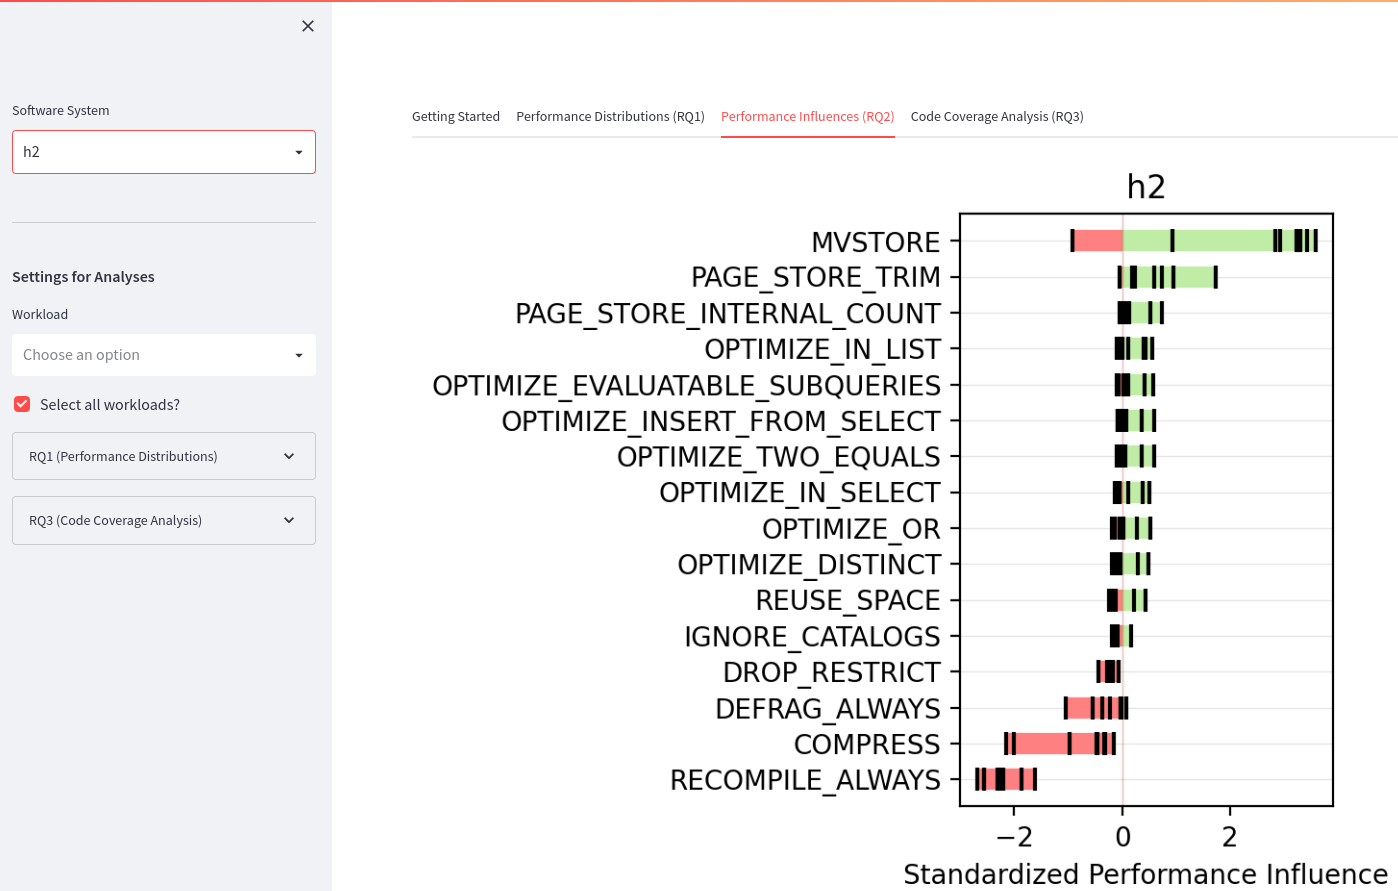
\includegraphics[width=0.95\linewidth]{images/rq2.png}
	\caption{Visualization of distribution of configuration influences across different different workloads for the database system \htwo.}
	\label{fig:dashboard}
\end{figure}

For demonstration, take as an example the visualization of distribution of configuration options' influences across different workloads for the database system \htwo presented in Fig.~\ref{fig:dashboard} using the dashboard. 
Via the topbar, one can select the type of analysis (correlation analysis of performance distributions, distribution of performance influences across workloads, and option-wise code coverage analysis). The sidebar allows for selecting a specific configuration option to analyze and tweaking further parameters for visualization. 


The dashboard is implemented using the \textsc{Python}
framework \texttt{streamlit} and is provided as a containerized
application (\textsc{Docker}) via the companion repository. This way, the dashboard not only complements the presentation of results in the study, but provides a means to reproduce analyses and reenact findings from our study.




